\documentclass{beamer}
\mode<presentation>

\usepackage{graphicx}

\usetheme{Singapore} % Dresden?
\title{A Simple Laboratory Environment \\for Real-World Offensive Security Education}
\author{Maxim Timchenko \and David Starobinski}
\institute{Electrical and Computer Engineering Department\\Boston University}
\date{SIGCSE'15, March 7, 2015}
\begin{document}
	\begin{frame}
		\titlepage
	\end{frame}
	
	\begin{frame}{Speaker}
		\begin{itemize}
			\item Lab assistant for \emph{Cybersecurity} course, Fall 2013
			\item TA for \emph{Cybersecurity} course, Fall 2014
			\item 120 students
			\item 3 professors, 3 sets of topics
			\item Different environments, assignments, approaches
		\end{itemize}
	\end{frame}
	
	\begin{frame}
		\titlepage
	\end{frame}
	
	\section{Our Goal}
	\subsection{Goal}
	\begin{frame}{``Offensive''?}
		\begin{center}
			
\includegraphics[width=0.6\textwidth]{parental-advisory-wikipedia.png}
		\end{center}
	\end{frame}
	
	\begin{frame}{``Offensive''}
		\begin{itemize}
			\item Attacker mindset vs. developer mindset
			\begin{itemize}
				\item ``How can I make this do something else''?
				\item Low-level, in-depth understanding
				\item Challenge bad assumptions
			\end{itemize}
			\vfill
			\item Both sides of the coin
			\begin{itemize}			
				\item Looking only at defense makes attacks ``abstract''
				\item Immediate reaction to trying attacks out
				\item Then, discuss how to defend
			\end{itemize}		
			\vfill		
			\item Students love it!
		\end{itemize}
	\end{frame}

	\begin{frame}{``Real-world''}
		\begin{itemize}
			\item Use the tools commonly used within the industry	
			\begin{itemize}			
				\item Practical experience
				\item Reuse
				\item Plenty of reference information
			\end{itemize}				
			\item Discuss actual exploits, demonstrate issues vividly
			\begin{itemize}
				\item Metasploit modules
				\item Social engineering
			\end{itemize}
			\item Cover current events (e.g. 2014: Shellshock)
		\end{itemize}		
	\end{frame}

	\begin{frame}{``Laboratory Environment''}
		\begin{itemize}
			\item Security
			\item Isolation
			\item Hardware Independence
		\end{itemize}			
	\end{frame}

	\begin{frame}{``Simple''}
		\begin{itemize}
			\item Reuse available components
			\item Simple to install and use
			\item Resource efficient
		\end{itemize}	
	\end{frame}

	\section{Related Work}
	\subsection{dummy name}
	\begin{frame}{Environments}
		Local isolated network containing actual hardware
		\vfill
		\begin{columns}
 		\begin{column}{0.5\textwidth}
    			\begin{itemize}
        				\item Expensive
        				\item Limited flexibility
        				\item Limited sharing
        				\item Resettable?
    			\end{itemize}
  		\end{column}

		\begin{column}{0.5\textwidth}
     			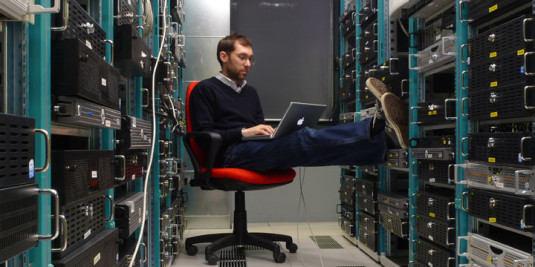
\includegraphics[width=\textwidth]{env-datacenter_rizzi.jpg}
			
			{\tiny Photo: Leonardo Rizzi, Flickr, Creative Commons}
  		\end{column}
		\end{columns}
	\end{frame}
	
	\begin{frame}{Environment Virtualization}
		\begin{block}{Centralized On Premises}
			\only<1>{
            		\begin{columns}
             		\begin{column}{0.5\textwidth}
                			\begin{itemize}
                    			\item Set-up and maintenance
                    			\item Scaling?
                    			\item Bandwidth requirements
					\item Example: Tele-Lab [10]
                			\end{itemize}
              		\end{column}
            
            		\begin{column}{0.5\textwidth}
				\begin{center}
                 		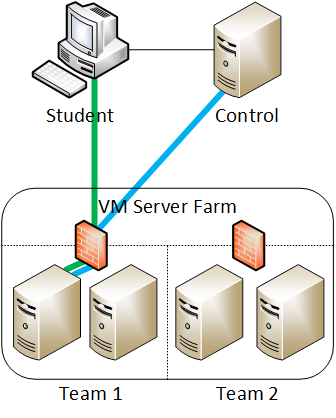
\includegraphics[width=0.6\textwidth]{centralized-virt.png}
				\end{center}
              		\end{column}
            		\end{columns}
			}
		\end{block}
		\begin{block}{Cloud}
			\only<2>{
            		\begin{columns}
             		\begin{column}{0.5\textwidth}
                			\begin{itemize}
                    			\item Administration
					\item Complicated architecture
                    			\item Cost!
                    			\item Potentially, worst responsiveness\\(traffic and delay)
					\item Example: Salah [6] on AWS
                			\end{itemize}
              		\end{column}
            
            		\begin{column}{0.5\textwidth}
						\begin{center}
                 		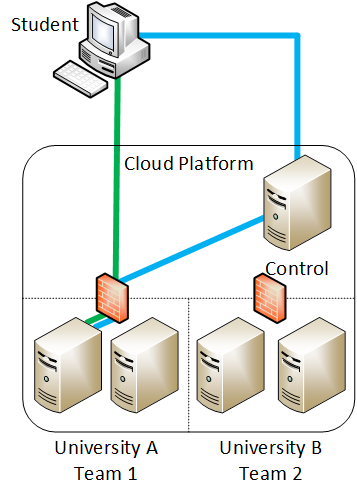
\includegraphics[width=0.6\textwidth]{cloud-virt.png}
				\end{center}
              		\end{column}
            		\end{columns}		
			}
		\end{block}
		\begin{block}{Local}
			\only<3>{
            		\begin{columns}
             		\begin{column}{0.5\textwidth}
                			\begin{itemize}
                    			\item Easy set-up
                    			\item No scaling issues
                    			\item Best responsiveness
                			\end{itemize}
              		\end{column}
            
            		\begin{column}{0.5\textwidth}
				\begin{center}
                 		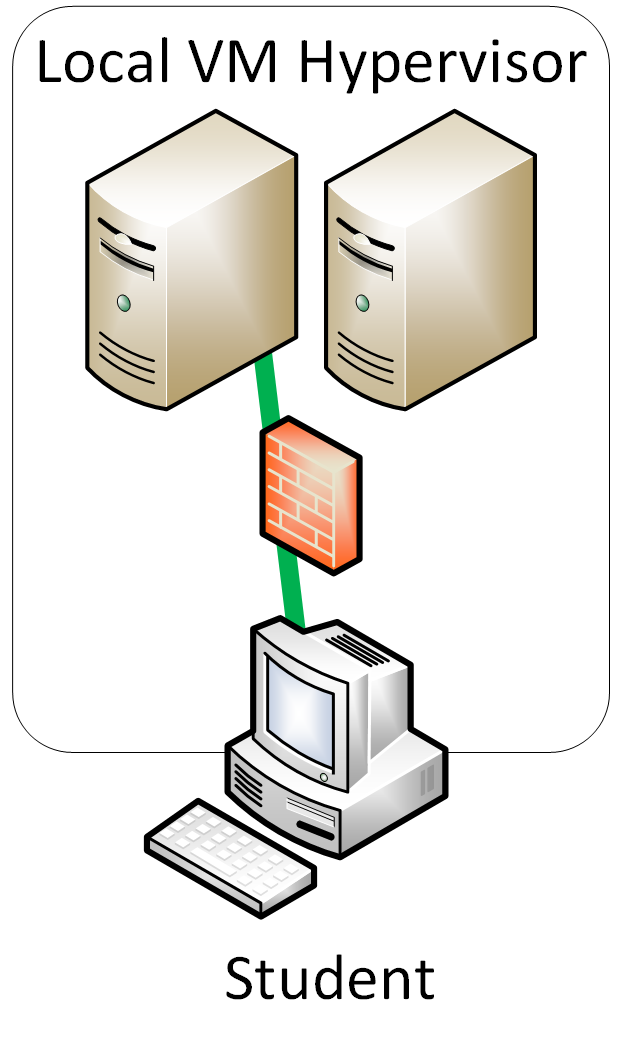
\includegraphics[width=0.4\textwidth]{local-virt.png}
				\end{center}
              		\end{column}
            		\end{columns}		
			}	
		\end{block}		
	\end{frame}	
	
	\begin{frame}{Existing Lab Sets}
		\begin{itemize}	
			\item The SEED project [2]
			\begin{itemize}	
				\item Comprehensive, but not a lot of overlap in topics (!)
				\item Exploratory in nature
			\end{itemize}		
			\item OWASP Hackademic [5]
			\begin{itemize}	
				\item Web applications security
				\item More elaborate setup required
			\end{itemize}
			\item Many papers with one or two labs
			\begin{itemize}	
				\item Reconciling environments, writing styles...
				\item Difficult to refer to previous material
			\end{itemize}
			\item Internet sources, e.g. ``How to use Metasploitable to hack X''
			\begin{itemize}
				\item Usually very narrow in scope and with poor style
				\item A walkthrough, not an assignment
			\end{itemize}
		\end{itemize}	
	\end{frame}
	
	\section{Contribution}	
	\subsection{dummy-name}

	\begin{frame}{Detailed Environment Architecture}
		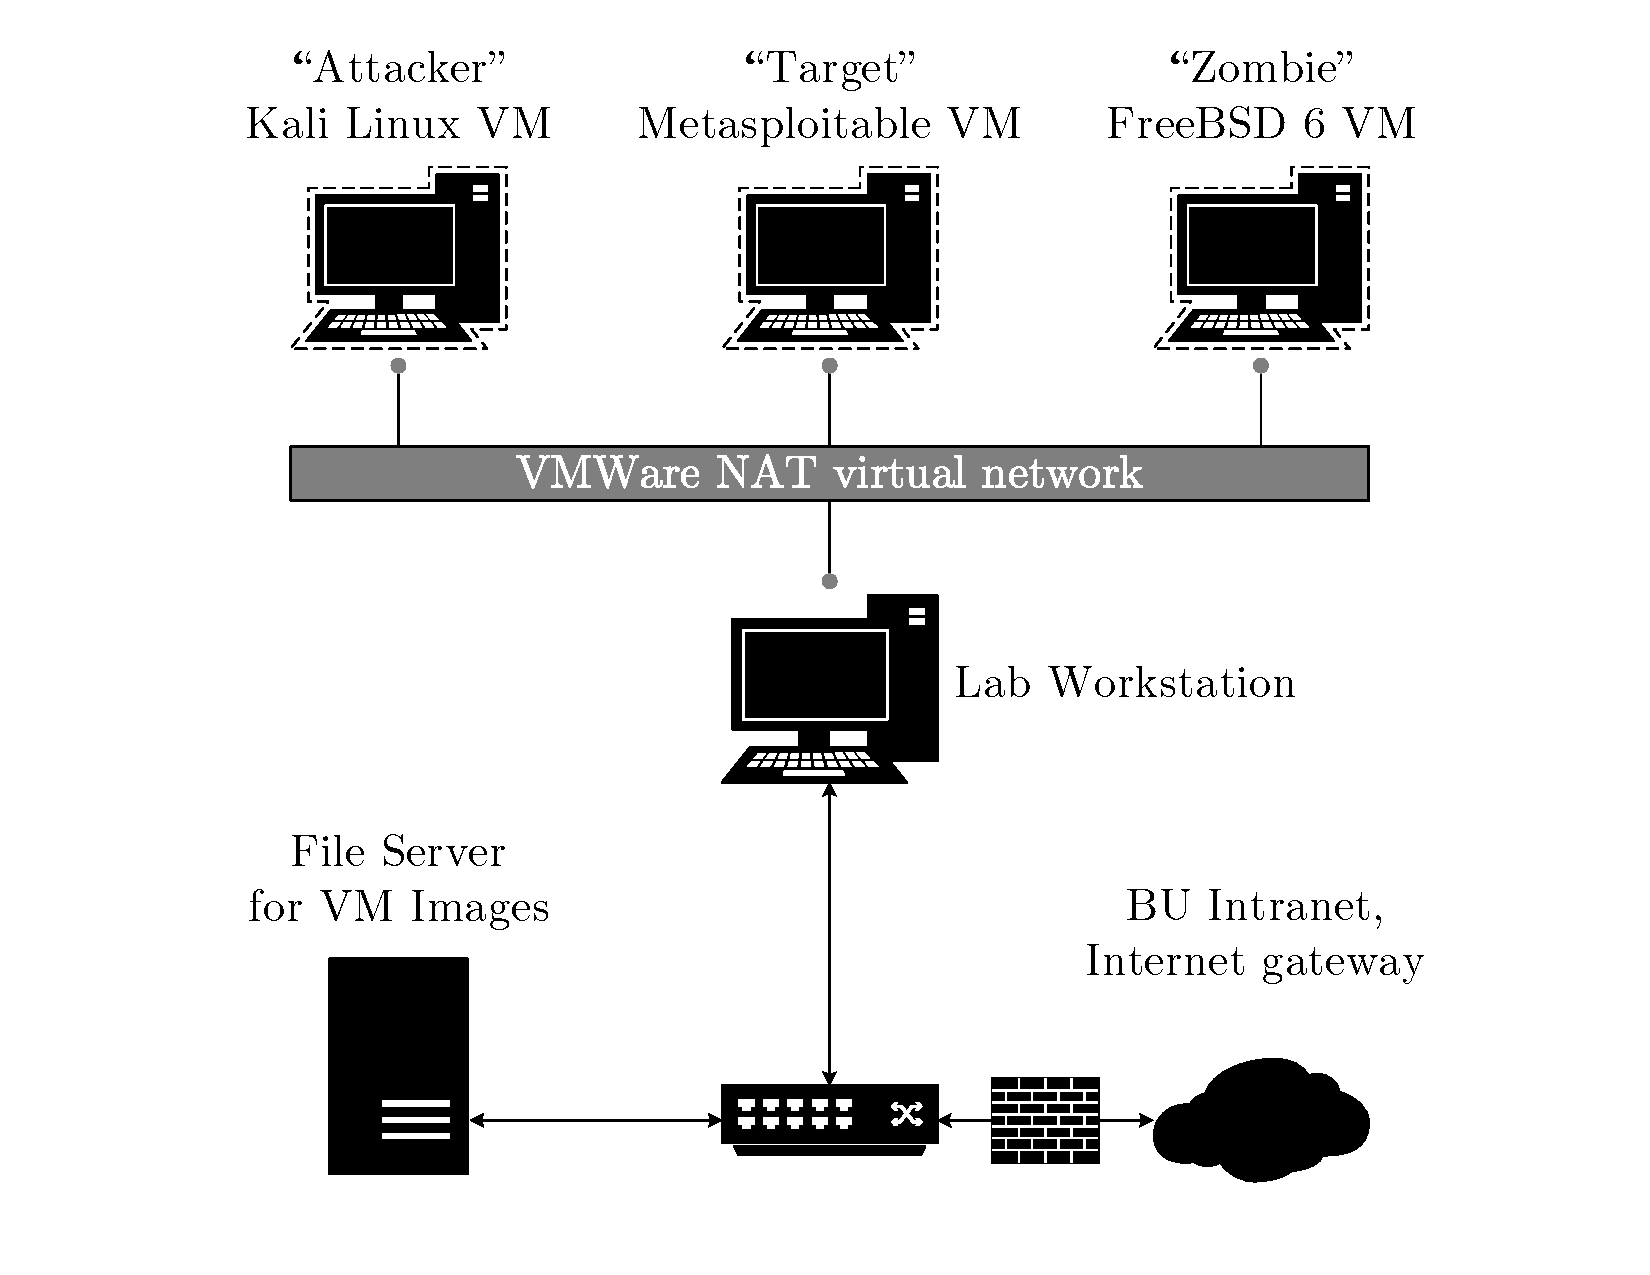
\includegraphics[page=1,width=\textwidth]{../paper/ec521_hostmap.pdf}
	\end{frame}

	\begin{frame}{VM Image Sets}
		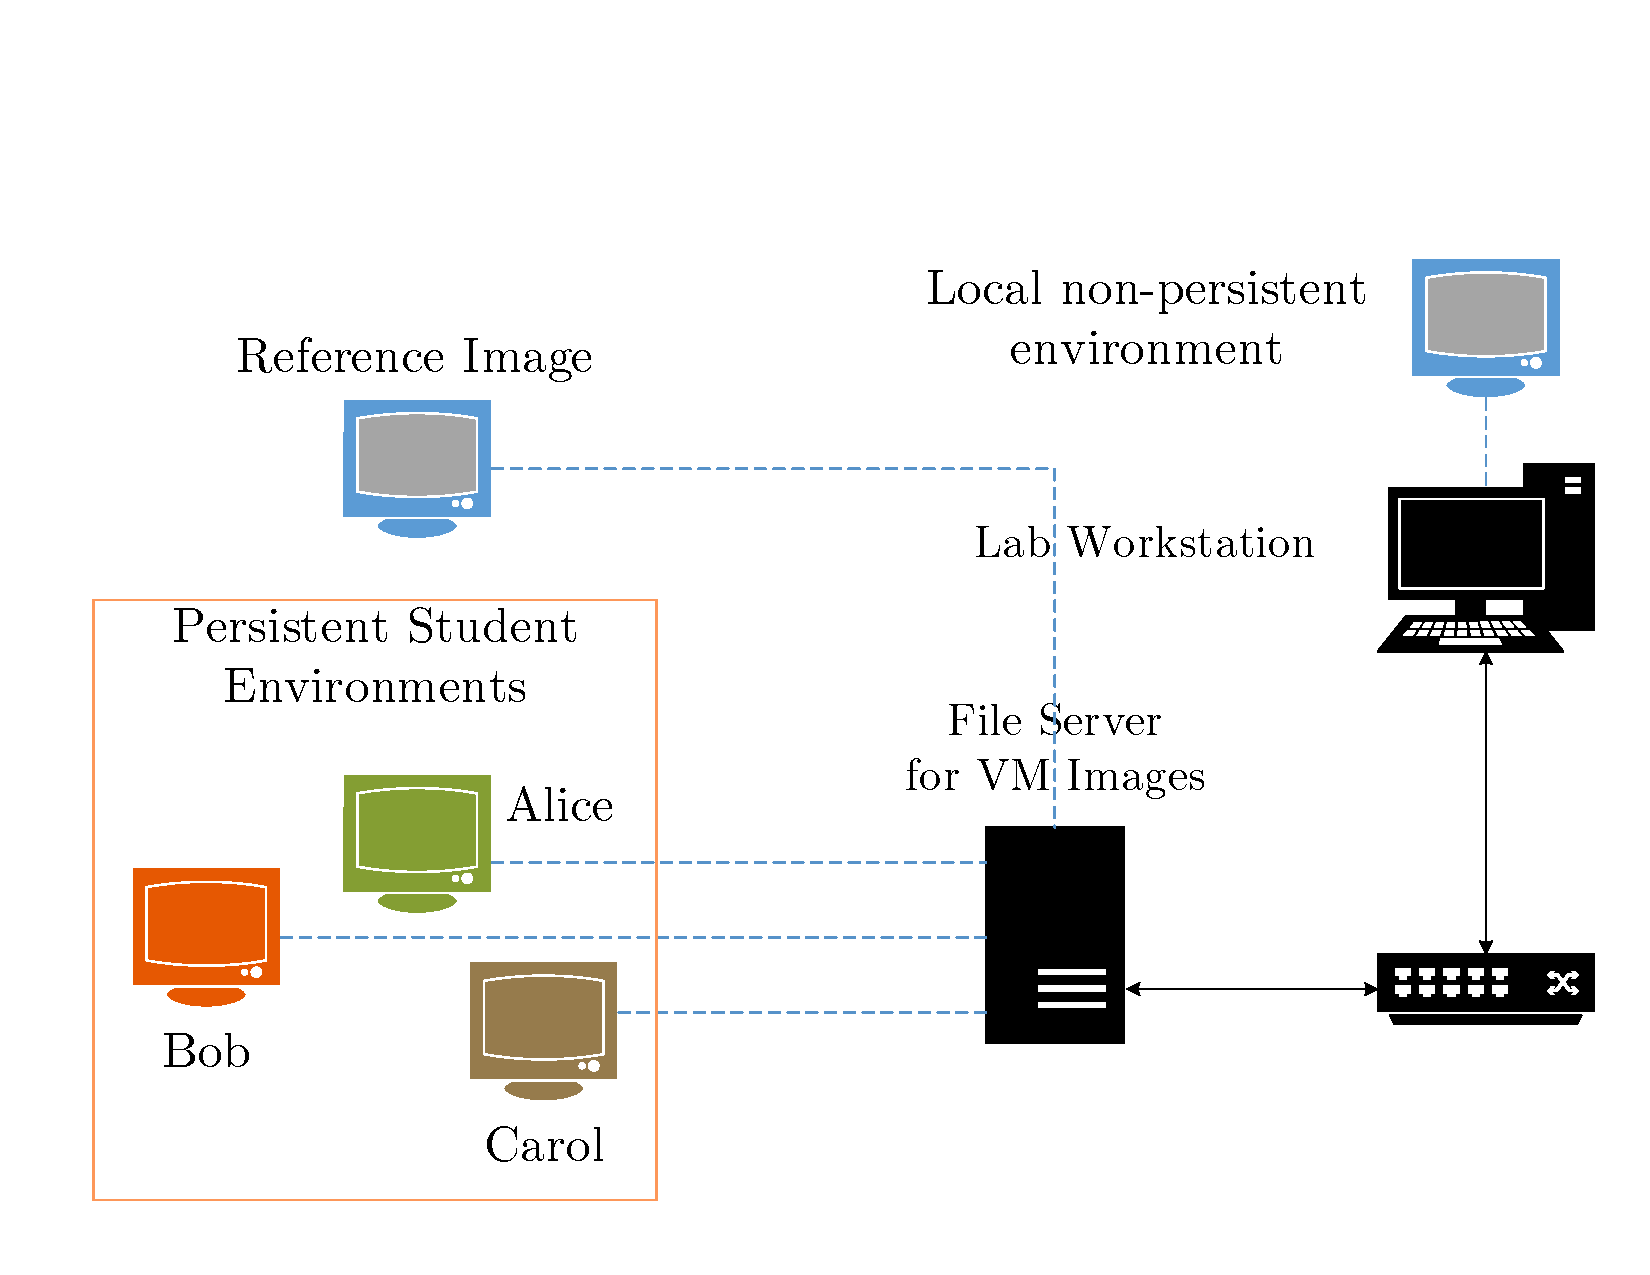
\includegraphics[page=1,width=\textwidth,clip=true, trim=0 0 0 1in]{vm-image-sets.pdf}
	\end{frame}

	\begin{frame}{Resource Requirements}
		\includegraphics[page=2,width=\textwidth, clip=true, trim=0.5in 6in 1in 0.5in]{Resources.pdf}
	\end{frame}
		
	\begin{frame}{Studying Cybersecurity Anywhere}
		\begin{center}
		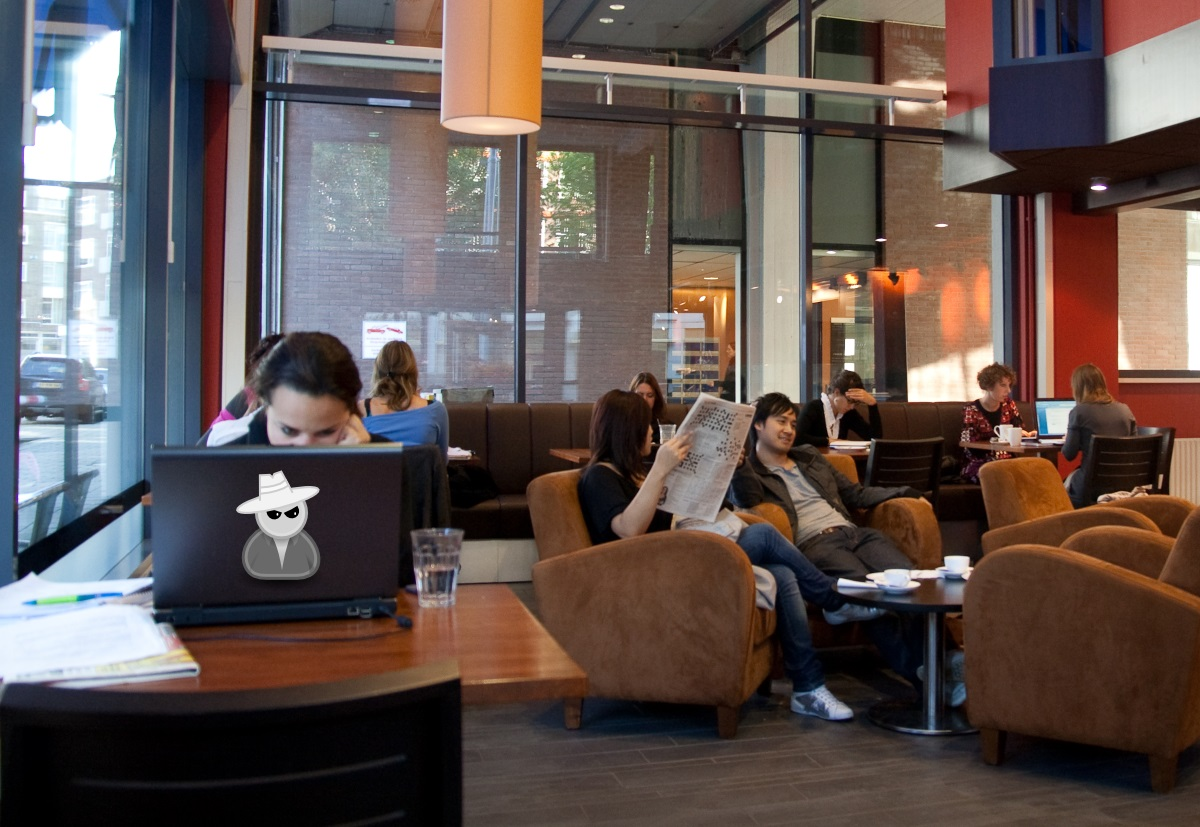
\includegraphics[width=0.8\textwidth]{coffeeshop_whitehat.jpg}
		
		{\tiny Photo: Alper Cugun, Flickr, CC-BY 2.0 | Whitehat Icon: Open Security Architecture, CC-BY-SA}
		\end{center}
	\end{frame}
			
	\begin{frame}{Future Work}
		\begin{itemize}	
			\item Item
		\end{itemize}
	\end{frame}

	\section{Summary}
	\subsection{dummy-name}	
	\begin{frame}{Summary}
		\begin{itemize}
			\item	A virtual-machine based environment for teaching cybersecurity
			\begin{itemize}			
				\item Requires no additional infrastructure
				\item Runs well on current hardware, including laptops
			\end{itemize}	
			\pause			
			\item A set of labs based on the environment
			\begin{itemize}			
				\item A choice of topics for an introductory course
				\item Structured, more guidance / less exploratory
				\item Try to build each lab on previous ones to reinforce
			\end{itemize}	
			\pause
			\item Directions for future work
			\begin{itemize}			
				\item Automated grading a prerequisite for scaling
				\item How to maintain the VMs going forward?
				\item More architectures (mobile/embedded) and network devices (SDN)
			\end{itemize}								
		\end{itemize}
	\end{frame}
	
	\begin{frame}{Thank you for your attention!}
		The sources for this talk and several of the labs can be found in our GitHub repository:
		\vfill
		\begin{center}
		\url{https://github.com/maxvt/cyberlabs}
		\end{center}
		\vfill
		Contact the authors at:
		\begin{itemize}
			\item \texttt{staro@bu.edu}
			\item \texttt{maxvt@bu.edu}, 
\includegraphics[width=9pt]{Twitter_bird_logo_2012.png}\hspace{0.2em}\texttt{@maxvt}
			\item \url{http://nislab.bu.edu/}
		\end{itemize}	
	\end{frame}
\end{document}